\documentclass[10pt,a4paper]{report}
\usepackage[latin1]{inputenc}
%\usepackage[utf8x]{inputenc}
\usepackage{amsmath}
\usepackage{amsfonts}
\usepackage{amssymb}
\usepackage{graphicx}
\usepackage[left=1.5cm,right=1.5cm,top=2.5cm,bottom=2.5cm]{geometry}

\pagenumbering{gobble}

\DeclareMathOperator{\ind}{\perp \!\!\! \perp}



% Le document est sur 6 pages organis�es comme ci-dessous :
% 1 3 5
% 2 4 6
\begin{document}

\begin{center}
\resizebox{\linewidth}{!}{\itshape \textbf{Generalization and}}
\end{center}
\vspace{80pt}

\begin{center}
\Huge{\textit{Introduction}}
\end{center}
\vspace{20pt}

\Large{
	
	Hidden Markov Models (HMMs) are widely used for probabilistic models of time series data. Here we used a generalization of HMMs by having observations depending from several parallel hidden Markov models (figure (a)). This factorization leads to a big time improvement when computing the EM algorithm, especially when the HMM has states taking many values.
	\newline
	\newline
	
	}

\begin{figure}[h]
	\centering
	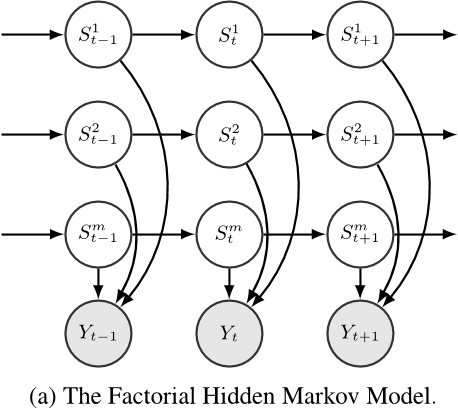
\includegraphics[width=0.7\textwidth]{fHMM.png}
	%\centerline{Factorial Hidden Markov Model}
	\label{fig:b}
\end{figure}


\newpage
\begin{center}
\Huge{\textit{The models}}
\end{center}












\newpage
\begin{center}
\resizebox{\linewidth}{!}{\itshape \textbf{acceleration of HMMs}}
\end{center}
\vspace{5pt}
\begin{center}
	\LARGE{Matthieu Jedor \& Alban Pierre}
	\vspace{15pt}
	
	\Large{Keywords: Hidden Markov models, time series, EM algorithm, graphical models, Bayesian networks, mean field
theory}
\end{center}
\vspace{30pt}
\begin{center}
\Huge{\textit{Experiments on synthetic data}}
\end{center}

\newpage
-










\newpage
\begin{center}
\resizebox{\linewidth}{!}{\itshape \textbf{using factorial HMMs}}
\end{center}
\vspace{80pt}
\begin{center}
\Huge{\textit{Experiments on real data}}
\end{center}

\newpage
-





\iffalse

\begin{figure}[h]
	\centering
	\includegraphics[width=1.0\textwidth]{P2.png}
	\centerline{Param�tres utilis�s pour calculer les probabilit�s des �tats cach�s}
	\label{fig:b}
\end{figure}


\begin{tabular}{lcc}
	& Entrainement & Test \\
	EM mixture de gaussiennes & -2371 & -2453 \\
	EM chaine de Markov cach�e & -1899 & -1957 \\
\end{tabular}
\newline

\fi

\end{document}
